\documentclass[a4paper,10pt]{article}

\usepackage[english]{babel}
\usepackage{graphicx}
\usepackage[colorlinks, linkcolor=black, citecolor=black, urlcolor=black]{hyperref}
\usepackage{geometry}
\geometry{tmargin=3cm, bmargin=2.2cm, lmargin=2.2cm, rmargin=2cm}
\usepackage{todonotes} %Used for the figure placeholders
\usepackage{ifthen}
\usepackage{pgfplots}
\pgfplotsset{compat=1.18}
\usepackage{pgfplots}
\usepackage{listings}
\usepackage{float}
\usepackage{xcolor} % good practice to load this explicitly before using \color
\usepackage{url} % of \usepackage{hyperref}

% Your name and student number must be filled in on the title page found in
% titlepage.tex.
\lstdefinelanguage{CUDA}{
  language=C++,
  morekeywords={
    __global__, __device__, __host__, __shared__, __constant__,
    __syncthreads, __threadfence_block, __threadfence, __threadfence_system,
    threadIdx, blockIdx, blockDim, gridDim
  },
  sensitive=true
}

% Algemene stijl
\lstset{
  language=CUDA,            % Use custom defined language
    basicstyle=\ttfamily\footnotesize,      % Monospaced font, small
    keywordstyle=[1]\color{blue}\bfseries,  % Mnemonics in blue and bold
    keywordstyle=[2]\color{purple},         % Registers in purple
    keywordstyle=[3]\color{brown}\bfseries, % Labels in brown and bold
    keywordstyle=[4]\color{teal}\bfseries,  % Constants and preprocessor in teal
    commentstyle=\color{gray},              % Comments in gray
    stringstyle=\color{red},                % Strings in red
    numbers=left,                           % Line numbers on the left
    numberstyle=\tiny\color{gray},          % Line number style
    stepnumber=1,                           % Line numbering step
    numbersep=5pt,                          % Space between line numbers and code
    breaklines=true,                        % Line breaking
    backgroundcolor=\color{gray!20},        % Light gray background
    frame=single,                           % Single frame around the code block
    captionpos=b,                           % Caption position at the bottom
    escapeinside={\%*}{*)},                 % Escape to LaTeX with %*...*)
}

\begin{document}
\newboolean{anonymize}
% Uncomment to create an anonymized version of your report
%\setboolean{anonymize}{true}

\begin{titlepage}
    \newpage
    \thispagestyle{empty}
    \frenchspacing
    \hspace{-0.2cm}
    \includegraphics[height=3.4cm]{sedes}
    \hspace{0.2cm}
    \rule{0.5pt}{3.4cm}
    \hspace{0.2cm}
    \begin{minipage}[b]{8cm}
        \Large{Katholieke\newline Universiteit\newline Leuven}\smallskip\newline
        \large{}\smallskip\newline
        \textbf{Department of\newline Computer Science}\smallskip
    \end{minipage}
    \hspace{\stretch{1}}
    \vspace*{3.2cm}\vfill
    \begin{center}
        \begin{minipage}[t]{\textwidth}
            \begin{center}
                \LARGE{\rm{\textbf{\uppercase{Advanced computer architecture}}}}\\
                \Large{\rm{project}}
            \end{center}
        \end{minipage}
    \end{center}
    \vfill
    \hfill\makebox[8.5cm][l]{%
        \vbox to 7cm{\vfill\noindent
            \ifthenelse{\boolean{anonymize}}{%
                {\rm \textbf{Anonymized}}\\
                {\rm Academic year 2025--2026}
            }{%
                {\rm \textbf{Thibaut Beck}}\\
                {\rm \textbf{Wannes Paesschesoone}}\\
              [2mm]
                {\rm Academic year 2025--2026}
            }
        }
    }
\end{titlepage}


\tableofcontents
\newpage
\section{Introduction}

This report talks about the implementation of a point cloud to voxel grid filter. The reason for implementing this filter is to reduce the number of points in a point cloud, while preserving the overall structure and appearance of the original data. Doing this on a CPU takes a long time for large point clouds, so the filter is implemented on a GPU using CUDA to take advantage of the parallel processing capabilities of modern graphics hardware.
\section{Theory}

\subsection{Point Cloud}
A \textbf{point cloud} is a collection of data points defined in a three-dimensional coordinate system.  
Each point represents a position in space, typically described by $(x, y, z)$ coordinates.  
Point clouds are commonly acquired using 3D scanners, LiDAR sensors, or photogrammetry systems.  
They are used in applications such as 3D modeling, robotics, mapping, and computer vision.

\subsection{Voxel}
A \textbf{voxel} (volumetric pixel) is the smallest unit of a 3D grid, similar to how a pixel is the smallest unit of a 2D image.  
Voxels divide 3D space into uniform cubes, allowing volumetric representations of shapes or environments.  
They are used in 3D reconstruction, simulation, gaming, and medical imaging.

\subsection{Pointcloud to Voxel Grid Filtering}
\textbf{Pointcloud to voxel grid filtering} converts an unstructured point cloud into a regular 3D grid.  
Space is divided into equal-sized voxels, and each point is assigned to its corresponding voxel.  
This reduces data density, removes redundant points, and creates a structured representation that is easier and faster to process for tasks such as downsampling and spatial queries.

\subsection{Morton Codes}
\textbf{Morton codes} (also called Z-order curves) are a method of encoding multi-dimensional coordinates into a single integer value.  
They work by bit-interleaving the binary coordinates (e.g., $x$, $y$, $z$).  
This encoding preserves spatial locality, making it useful for data structures such as octrees and for accelerating spatial queries on GPUs.

\subsection{CUDA Thrust Library}
The \textbf{CUDA Thrust library} is a parallel algorithms library for NVIDIA GPUs.  
It provides high-level abstractions similar to the C++ Standard Template Library (STL), including parallel sorting, scanning, reduction, and vector operations.  
Thrust simplifies GPU programming by offering ready-to-use, highly optimized parallel primitives.

\subsection{LAS Files}
\textbf{LAS files} are a standardized file format used for storing LiDAR point cloud data.  
The format supports 3D coordinates, intensity values, classification labels, GPS time, color information, and other metadata.  
LAS is widely used in geospatial applications, surveying, and remote sensing due to its efficiency and interoperability.



\section {Voxel size}
The voxel size is an important parameter in the point cloud to voxel filter. The bigger the voxel size ,the more points will be grouped together into a single voxel, resulting in a coarser representation of the original point cloud. Conversely, a smaller voxel size will result in a finer representation, with more voxels and fewer points per voxel.

\section{Implementation}
In this chapter, the practical implementation details of the point cloud to voxel grid filter are presented. To leverage the massive parallelism of modern hardware, the algorithms were developed using CUDA for GPU acceleration. Two distinct parallel strategies were designed to solve the voxelization problem: a sorting-based approach using Morton encoding, and a scattering approach using a GPU-resident dynamic hash map. This hashmap uses the same Morton encoding for voxel indexing, ensuring consistency between both methods.
Both voxelizers share the same Morton encoding utilities so that a 3D voxel index is always mapped to the same 64-bit key, independent of the backend. On top of that, the Morton-and-sort voxelizer introduces its own per-voxel accumulation structure and reduction functor, while the hash-based implementation uses a dedicated hash bucket structure.

\subsection{Shared Morton Encoding Utilities}

\paragraph{Bit expansion helper.}
The first shared building block is the mapping from 3D integer voxel coordinates $(i_x,i_y,i_z)$ to a single 64-bit Morton code. This is reused in \emph{both} voxelizers: in the sorting-based pipeline it is used to generate keys for \texttt{thrust::sort\_by\_key}, while in the hash-based pipeline the same 64-bit Morton code serves directly as the hash key for open addressing.

The helper function \texttt{splitBy3} expands a 21-bit integer into a 64-bit value in which each original bit is separated by two zero bits:

\begin{lstlisting}[language=CUDA,caption={Bit expansion of a 21-bit coordinate into Morton layout (shared).}]
__device__ __host__ inline uint64_t splitBy3(uint64_t v) {
    v = (v | (v << 32)) & 0x1f00000000ffffULL;
    v = (v | (v << 16)) & 0x1f0000ff0000ffULL;
    v = (v | (v <<  8)) & 0x100f00f00f00f00fULL;
    v = (v | (v <<  4)) & 0x10c30c30c30c30c3ULL;
    v = (v | (v <<  2)) & 0x1249249249249249ULL;
    return v;
}
\end{lstlisting}

\paragraph{Morton code generation.}
Using \texttt{splitBy3}, the actual Morton code is formed by interleaving the expanded bits of the three coordinates:

\begin{lstlisting}[language=CUDA,caption={Morton encoding of 3D voxel indices (shared).}]
__device__ __host__ inline uint64_t mortonEncode(uint32_t x,
                                                 uint32_t y,
                                                 uint32_t z) {
    return (splitBy3((uint64_t)x) << 2) |
           (splitBy3((uint64_t)y) << 1) |
            splitBy3((uint64_t)z);
}
\end{lstlisting}

Both functions are marked \texttt{\_\_device\_\_ \_\_host\_\_ inline}, so they can be called from host-side test code as well as from all CUDA kernels in both voxelization backends.

\subsection{Morton and Sort Voxelizer}

To implement the Morton-and-sort voxelizer efficiently on the GPU, the pipeline is decomposed into: (i) Morton code generation via the shared utilities, (ii) per-voxel accumulation of point attributes, and (iii) CUDA kernels that bridge raw device arrays with Thrust's sort-and-reduce primitives. The accumulation structures and reduction functor described below are specific to this implementation and are \emph{not} used by the hash-based voxelizer.

\paragraph{Per-voxel accumulation structure.}
To compute voxel centroids and average colors in a single pass after sorting, we define a compact accumulation structure \texttt{PointAccum}. It stores the running sums of coordinates and RGB components, as well as the number of points that contributed to the voxel:

\begin{lstlisting}[language=CUDA,caption={Accumulation structure for voxel-wise reduction (Morton-and-sort only).}]
struct PointAccum {
    float    sumX, sumY, sumZ;
    uint32_t sumR, sumG, sumB;
    uint32_t count;
    
    __device__ __host__ PointAccum()
        : sumX(0), sumY(0), sumZ(0),
          sumR(0), sumG(0), sumB(0),
          count(0) {}

    __device__ __host__ PointAccum(float x, float y, float z,
                                   uint8_t r, uint8_t g, uint8_t b)
        : sumX(x), sumY(y), sumZ(z),
          sumR(r), sumG(g), sumB(b),
          count(1) {}
};
\end{lstlisting}

This structure is used as the value type in the subsequent reduction-by-key stage and is therefore only required by the sorting-based voxelizer.

\paragraph{Binary reduction functor.}
To use \texttt{PointAccum} with \texttt{thrust::reduce\_by\_key}, we define a binary functor \texttt{PointAccumOp}. It describes how two partial voxel accumulators are merged:

\begin{lstlisting}[language=CUDA,caption={Binary operator for reducing \texttt{PointAccum} values (Morton-and-sort only).}]
struct PointAccumOp {
    __device__ __host__
    PointAccum operator()(const PointAccum& a,
                          const PointAccum& b) const {
        PointAccum result;
        result.sumX  = a.sumX  + b.sumX;
        result.sumY  = a.sumY  + b.sumY;
        result.sumZ  = a.sumZ  + b.sumZ;
        result.sumR  = a.sumR  + b.sumR;
        result.sumG  = a.sumG  + b.sumG;
        result.sumB  = a.sumB  + b.sumB;
        result.count = a.count + b.count;
        return result;
    }
};
\end{lstlisting}

This functor is specific to the reduction-based pipeline and is not needed by the dynamic hash map implementation.

\paragraph{Morton code computation kernel.}
The first CUDA kernel in this voxelizer takes the input point positions and converts them into Morton codes using the shared \texttt{mortonEncode} helper. Each thread processes exactly one point:

\begin{lstlisting}[language=CUDA,caption={Kernel computing Morton codes for each point (Morton-and-sort).}]
__global__ void computeMortonCodesKernel(
    const float* x,
    const float* y,
    const float* z,
    uint64_t* mortonCodes,
    float minX, float minY, float minZ,
    float invVoxelSize,
    size_t numPoints)
{
    int idx = blockIdx.x * blockDim.x + threadIdx.x;
    if (idx >= numPoints) return;

    // Compute voxel indices (offset by min to ensure non-negative indices)
    uint32_t ix = (uint32_t)floorf((x[idx] - minX) * invVoxelSize);
    uint32_t iy = (uint32_t)floorf((y[idx] - minY) * invVoxelSize);
    uint32_t iz = (uint32_t)floorf((z[idx] - minZ) * invVoxelSize);

    mortonCodes[idx] = mortonEncode(ix, iy, iz);
}
\end{lstlisting}

The kernel assumes a structure-of-arrays (SoA) layout (\texttt{x}, \texttt{y}, \texttt{z} in separate buffers) for coalesced memory access. The inverse voxel size is precomputed on the host to avoid divisions in device code.

\paragraph{Accumulator creation kernel.}
After sorting the points by their Morton codes, a \texttt{PointAccum} object is created for each point in sorted order. Rather than physically reordering all input arrays, a separate index array encodes the permutation induced by the sort:

\begin{lstlisting}[language=CUDA,caption={Kernel creating \texttt{PointAccum} objects after sorting (Morton-and-sort).}]
__global__ void createPointAccumKernel(
    const float*  x,
    const float*  y,
    const float*  z,
    const uint8_t* r,
    const uint8_t* g,
    const uint8_t* b,
    const uint32_t* indices,
    PointAccum* accums,
    size_t numPoints)
{
    int idx = blockIdx.x * blockDim.x + threadIdx.x;
    if (idx >= numPoints) return;

    uint32_t origIdx = indices[idx];
    accums[idx] = PointAccum(
        x[origIdx], y[origIdx], z[origIdx],
        r[origIdx], g[origIdx], b[origIdx]
    );
}
\end{lstlisting}

\paragraph{Integration in the outer loop.}
The outer host function for the Morton-and-sort voxelizer (not shown in full) orchestrates the following steps:

\begin{enumerate}
    \item \textbf{Preprocessing:} Compute the global bounding box and \texttt{invVoxelSize} on the CPU.
    \item \textbf{Device setup:} Upload positions and colors to device vectors; initialize an index array with \texttt{thrust::sequence}.
    \item \textbf{Morton computation:} Launch \texttt{computeMortonCodesKernel} to fill the Morton code buffer using the shared \texttt{mortonEncode}.
    \item \textbf{Sorting:} Call \texttt{thrust::sort\_by\_key} on the pair \texttt{(d\_mortonCodes, d\_indices)}.
    \item \textbf{Accumulator creation:} Launch \texttt{createPointAccumKernel} to build a \texttt{PointAccum} per sorted point.
    \item \textbf{Reduction by voxel:} Invoke \texttt{thrust::reduce\_by\_key} with \texttt{PointAccum} values and \texttt{PointAccumOp} to obtain one accumulator per occupied voxel.
    \item \textbf{Final averaging:} Copy the reduced accumulators back to the host and divide sums by \texttt{count} to obtain centroid and color per voxel.
\end{enumerate}

\subsection{Dynamic Hash Map Voxelizer}

The second approach implements a custom open-addressing hash table directly in GPU global memory. This method is designed for maximum throughput, avoiding the global synchronization and $O(N \log N)$ complexity of the sorting-based pipeline. Instead of ordering points, it scatters them into a large hash table and accumulates voxel statistics in-place using atomics.

This implementation \emph{reuses} only the shared Morton encoding helpers (\texttt{splitBy3} and \texttt{mortonEncode}). The per-voxel accumulation is performed directly inside each hash bucket, so there is no need for \texttt{PointAccum} or \texttt{PointAccumOp}.

\paragraph{Hash bucket layout.}
Each entry in the GPU hash table is represented by a tightly packed \texttt{HashBucket} structure:

\begin{lstlisting}[language=CUDA,caption={Aligned hash bucket structure and empty key sentinel (hash voxelizer).}]
struct __align__(16) HashBucket {
    unsigned long long key;  // 64-bit Morton code
    float sumX, sumY, sumZ;
    uint32_t sumR, sumG, sumB;
    uint32_t count;
};

#define EMPTY_KEY 0xFFFFFFFFFFFFFFFFULL
\end{lstlisting}

The \texttt{\_\_align\_\_(16)} qualifier improves memory coalescing, and \texttt{EMPTY\_KEY} serves as a sentinel to identify unused slots. The 64-bit \texttt{key} field stores the Morton code computed by the shared \texttt{mortonEncode} function.

\paragraph{Hash table initialization.}
Before insertion, the hash table is cleared by setting all keys to \texttt{EMPTY\_KEY} and zeroing the accumulators:

\begin{lstlisting}[language=CUDA,caption={Kernel initializing the GPU hash table (hash voxelizer).}]
__global__ void initHashMapKernel(HashBucket* table, size_t capacity) {
    size_t idx = blockIdx.x * blockDim.x + threadIdx.x;
    if (idx < capacity) {
        table[idx].key   = EMPTY_KEY;
        table[idx].count = 0;

        table[idx].sumX = 0.0f;
        table[idx].sumY = 0.0f;
        table[idx].sumZ = 0.0f;
        table[idx].sumR = 0;
        table[idx].sumG = 0;
        table[idx].sumB = 0;
    }
}
\end{lstlisting}

\paragraph{Hash-Based Voxel Accumulation using Atomic Open Addressing}
The core function of the hash-based voxelizer is the $\texttt{populateHashMapKernel}$ CUDA kernel, which implements a scatter-and-accumulate pattern using a 64-bit Morton code derived from $3D$ integer coordinates $(i_x, i_y, i_z)$ via $\texttt{mortonEncode}$ as the key. Each thread calculates an initial hash slot $H = \texttt{mortonCode} \pmod{\texttt{capacity}}$ and uses linear probing to find the correct $\texttt{HashBucket}$. Concurrency is managed by atomically claiming an empty slot using $\texttt{atomicCAS}$ (Compare-and-Swap) with $\texttt{EMPTY\_KEY}$, or by finding a slot already containing its key. Once the correct slot is secured, the thread uses atomic additions ($\texttt{atomicAdd}$) to safely accumulate the point's properties (position sums, color sums, and $\texttt{count}$) into the shared $\texttt{HashBucket}$ structure, ensuring thread-safe data aggregation despite concurrent writes.
\begin{lstlisting}[language=CUDA,caption={Kernel inserting points into the GPU hash map (hash voxelizer).}]
__global__ void populateHashMapKernel(
    const float*   x, const float*   y, const float*   z,
    const uint8_t* r, const uint8_t* g, const uint8_t* b,
    HashBucket* table,
    size_t capacity,
    size_t numPoints,
    float minX, float minY, float minZ,
    float invVoxelSize)
{
    size_t idx = blockIdx.x * blockDim.x + threadIdx.x;
    if (idx >= numPoints) return;

    // 1. Quantize position to voxel grid and compute Morton key
    uint32_t ix = (uint32_t)floorf((x[idx] - minX) * invVoxelSize);
    uint32_t iy = (uint32_t)floorf((y[idx] - minY) * invVoxelSize);
    uint32_t iz = (uint32_t)floorf((z[idx] - minZ) * invVoxelSize);

    uint64_t mortonCode = mortonEncode(ix, iy, iz);

    // 2. Initial hash slot
    size_t hashIdx = mortonCode % capacity;

    // 3. Linear probing with atomic CAS and atomic adds
    for (size_t i = 0; i < capacity; ++i) {
        size_t currentSlot = (hashIdx + i) % capacity;

        unsigned long long oldKey = table[currentSlot].key;

        // Try to claim an empty slot
        if (oldKey == EMPTY_KEY) {
            unsigned long long assumed =
                atomicCAS((unsigned long long*)&table[currentSlot].key,
                          EMPTY_KEY,
                          (unsigned long long)mortonCode);
            if (assumed == EMPTY_KEY) {
                oldKey = mortonCode; // we now own this bucket
            } else {
                oldKey = assumed;    // another thread claimed it
            }
        }

        // If this bucket belongs to our Morton key, accumulate data
        if (oldKey == mortonCode) {
            atomicAdd(&table[currentSlot].sumX, x[idx]);
            atomicAdd(&table[currentSlot].sumY, y[idx]);
            atomicAdd(&table[currentSlot].sumZ, z[idx]);

            atomicAdd(&table[currentSlot].sumR, (uint32_t)r[idx]);
            atomicAdd(&table[currentSlot].sumG, (uint32_t)g[idx]);
            atomicAdd(&table[currentSlot].sumB, (uint32_t)b[idx]);

            atomicAdd(&table[currentSlot].count, 1);
            return;
        }

        // Otherwise: collision with a different key, continue probing
    }
}
\end{lstlisting}

Note that this kernel does \emph{not} use \texttt{PointAccum} or \texttt{PointAccumOp}; all aggregation happens directly inside the \texttt{HashBucket}.

\paragraph{Counting valid voxels.}
Because open addressing leaves gaps in the hash table, a compaction pass is required. The first step is to count how many buckets are actually occupied:

\begin{lstlisting}[language=CUDA,caption={Kernel counting the number of occupied buckets (hash voxelizer).}]
__global__ void countValidBucketsKernel(
    HashBucket* table,
    size_t capacity,
    uint32_t* counter)
{
    size_t idx = blockIdx.x * blockDim.x + threadIdx.x;
    if (idx < capacity) {
        if (table[idx].key != EMPTY_KEY) {
            atomicAdd(counter, 1);
        }
    }
}
\end{lstlisting}

\paragraph{Collecting results.}
A second pass converts the populated buckets into a dense array of voxel representatives. As in the sorting-based implementation, each voxel is represented by its centroid and average color:

\begin{lstlisting}[language=CUDA,caption={Kernel converting hash buckets into final voxel points (hash voxelizer).}]
__global__ void collectResultsKernel(
    HashBucket* table,
    size_t capacity,
    Point* output,
    uint32_t* globalCounter)
{
    size_t idx = blockIdx.x * blockDim.x + threadIdx.x;
    if (idx >= capacity) return;

    HashBucket bucket = table[idx];

    if (bucket.key != EMPTY_KEY && bucket.count > 0) {
        uint32_t outIdx = atomicAdd(globalCounter, 1);

        float c = (float)bucket.count;

        Point p;
        p.x = bucket.sumX / c;
        p.y = bucket.sumY / c;
        p.z = bucket.sumZ / c;
        p.r = (uint8_t)(bucket.sumR / bucket.count);
        p.g = (uint8_t)(bucket.sumG / bucket.count);
        p.b = (uint8_t)(bucket.sumB / bucket.count);

        output[outIdx] = p;
    }
}
\end{lstlisting}

\paragraph{Integration in the outer loop.}
The host-side driver for the dynamic hash map voxelizer can then be summarized as:

\begin{enumerate}
    \item \textbf{Capacity selection:} Choose a hash table capacity as a multiple of the number of points (e.g.\ factor 2--4).
    \item \textbf{Preprocessing:} Compute the bounding box and \texttt{inverse VoxelSize} on the CPU.
    \item \textbf{Device setup:} Allocate device arrays for point attributes and copy input data.
    \item \textbf{Hash table initialization:} Allocate and clear \texttt{HashBucket} array via \texttt{initHashMapKernel}.
    \item \textbf{Scatter-and-accumulate:} Launch \texttt{populateHashMapKernel}, which uses the shared \texttt{mortonEncode} to derive keys and accumulates directly into buckets.
    \item \textbf{Voxel counting:} Use \texttt{countValidBucketsKernel} to determine the number of occupied buckets and allocate a dense output array.
    \item \textbf{Compaction:} Reset the counter and call \texttt{collectResultsKernel} to write voxel centroids and colors into the dense output array.
    \item \textbf{Host transfer:} Copy the compact output back to the CPU and release GPU memory.
\end{enumerate}

In this way, the two voxelizers share a single, consistent Morton encoding implementation, while each maintains its own accumulation and reduction strategy tailored to its parallelization scheme.
\section{Results and Analysis}
\subsection{Timing remarks and methodology}
All the following results were obtained on relatively old hardware: a NVIDIA Geforce GTX 1080ti with 11GB of GDDR5X memory, paired with an Intel Core i7-8700K CPU @ 4.8 GHz and 32GB of DDR4 RAM and the pc runs ubuntu 24.04.3 LTS. The point cloud used for testing contains 648433 points, representing a dense scan of an urban environment.
\subsection{General Observations}
The voxelizers are compared among five voxel sizes (0.25, 0.5, 0.75, 1.0, 1.25). For each voxel size, eight block sizes were tested (1, 2, 4, 8, 16, 32, 64, 256, 512, 1024 threads per block). The hash-table voxelizer was evaluated with three different capacity factors (2, 3, and 4 times the number of input points). The performance metrics recorded include total execution time and a breakdown of time spent in key phases of each algorithm.
Every configuration was run 100 times to obtain an average execution time, minimizing the impact of transient system load variations.

\subsection{Performance Analysis per Method}

\subsubsection{Morton-Code Voxelizer}
The Morton-based approach demonstrates consistent and predictable performance. Key findings include:

\begin{itemize}
    \item \textbf{Optimal block size:} 4--256 threads per block.
    \item \textbf{Total execution time:} Ranging from 25.18\,ms (voxel size 1.25, block size 64) to 40.46\,ms (voxel size 0.25, block size 1).
    \item \textbf{Primary bottleneck:} The sorting stage dominates runtime, requiring approximately 0.90--1.02\,ms, nearly constant across all tests.
\end{itemize}

Very small block sizes (1--4 threads) significantly slow down Morton-code generation (0.27--1.07\,ms), while larger block sizes stabilize this step to around 0.04\,ms.

\subsubsection{Hash-Table Voxelizer}
The hash-based method demonstrates greater variability, largely influenced by the selected capacity factor of the hash table.

\paragraph{Capacity Factor 2 (highest efficiency)}
\begin{itemize}
    \item \textbf{Best overall performance:} 25.67\,ms (voxel size 1.0, block size 32).
    \item \textbf{Optimal block sizes:} 8--32 threads per block.
    \item \textbf{Advantages:} Lowest memory overhead and fastest device-to-host transfer times.
\end{itemize}

\paragraph{Capacity Factor 3 (balanced)}
\begin{itemize}
    \item Execution times are \textbf{2--4\,ms slower} compared to capacity factor 2.
    \item Reduced collisions during accumulation, at the cost of increased memory usage.
\end{itemize}

\paragraph{Capacity Factor 4 (highest overhead)}
\begin{itemize}
    \item \textbf{5--10\,ms slower} than capacity factor 2.
    \item Initialization and memory operations increase disproportionately.
    \item Device-to-host + cleanup time rises up to 5.26\,ms (compared to 2.71\,ms for CF=2).
\end{itemize}

\subsection{Impact of Voxel Size}
Smaller voxel sizes generate a significantly larger number of unique voxel entries. This favors the hash-table method with a low capacity factor, as the Morton approach becomes less efficient when spatial data is highly fragmented.

For larger voxels (e.g., voxel size 1.25), the Morton method benefits from predictable spatial coherence and memory access patterns, making it more efficient than the hash-based approach.

\subsection{Impact of Block Size}
\begin{itemize}
    \item \textbf{Block sizes 1--4:} Strong performance penalties due to insufficient warp utilization.
    \item \textbf{Block sizes 8--256:} Optimal performance range with minimal overhead.
    \item \textbf{Block sizes 512--1024:} No significant improvements; potentially limited by register pressure.
\end{itemize}

\subsection{Timing Breakdown}

\subsubsection{Morton Method}
Dominant phases:
\begin{enumerate}
    \item \textbf{Sorting:} 0.90--1.02\,ms (consistent across tests)
    \item \textbf{Morton code computation:} 0.04--1.07\,ms (strongly dependent on block size)
    \item \textbf{Point accumulation:} 0.24--1.08\,ms
\end{enumerate}

\subsubsection{Hash Method}
Dominant phases:
\begin{enumerate}
    \item \textbf{Device-to-host transfer + cleanup:} 2.71--5.26\,ms (increases with capacity factor)
    \item \textbf{Initialization:} 0.33--3.71\,ms (proportional to hash-table size)
    \item \textbf{Populate phase:} 0.31--2.46\,ms (collision-sensitive)
\end{enumerate}

\subsection{Conclusions}

\subsubsection{Optimal Configurations}
The analysis indicates that different voxel sizes benefit from different GPU strategies:

\begin{itemize}
    \item \textbf{Small voxel sizes (0.25--0.5):} Hash-based voxelizer with capacity factor 2 and a block size of 16--32 threads.
    \item \textbf{Medium voxel sizes (0.75--1.0):} Hash-based voxelizer with capacity factor 2 and a block size of 32 threads.
    \item \textbf{Large voxel sizes (1.25 and above):} Morton-code voxelizer with a block size between 64 and 256 threads.
\end{itemize}

\subsubsection{Explanation}
These optimal configurations follow from the observed behaviour of both voxelization methods:

\begin{enumerate}
    \item For small voxel sizes, the hash method with capacity factor 2 achieves the highest throughput due to low memory overhead and efficient device-to-host transfers.
    \item For larger voxel sizes, the Morton-based approach becomes more efficient thanks to spatial coherence and predictable memory access patterns.
    \item Block sizes between 16 and 64 threads provide the most balanced performance in terms of occupancy and register usage.
\end{enumerate}

\subsubsection{Performance Limitations}
Despite their strengths, both methods exhibit certain limitations:

\begin{itemize}
    \item The hash-based method is primarily constrained by memory bandwidth, especially during device-to-host transfers.
    \item The Morton-based method is strongly dominated by the sorting stage, which forms its main computational bottleneck.
    \item For both approaches, increasing block sizes beyond 256 threads yields minimal benefits due to hardware saturation.
\end{itemize}

\subsection {gpu vs cpu performance}
\textbf{TODOOOOOOOOOOOOOOOOOOOOOOOOOO}


% Requires pgfplots package
% Add to preamble: \usepackage{pgfplots}
% \pgfplotsset{compat=1.17}

% GRAPH 1: Voxel Size 0.25
\begin{figure}[H]
\centering
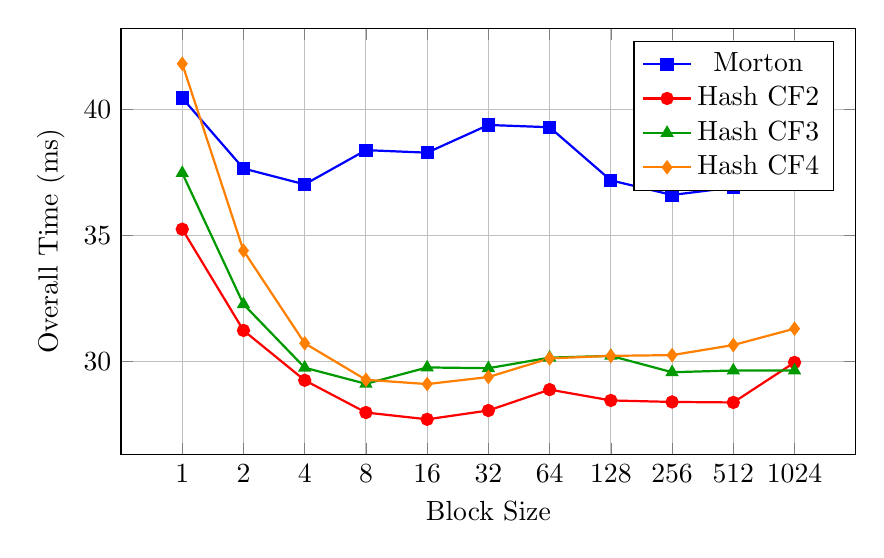
\begin{tikzpicture}
\begin{axis}[
    width=0.9\textwidth,
    height=7cm,
    xlabel={Block Size},
    ylabel={Overall Time (ms)},
    legend pos=north east,
    xmode=log,
    log basis x={2},
    xtick={1,2,4,8,16,32,64,128,256,512,1024},
    xticklabels={1,2,4,8,16,32,64,128,256,512,1024},
    grid=major,
    mark size=2pt,
]

% Morton
\addplot[color=blue,mark=square*,thick] coordinates {
    (1,40.46) (2,37.66) (4,37.03) (8,38.39) (16,38.29) 
    (32,39.39) (64,39.30) (128,37.19) (256,36.61) (512,36.91) (1024,39.67)
};

% Hash CF2
\addplot[color=red,mark=*,thick] coordinates {
    (1,35.25) (2,31.23) (4,29.25) (8,27.97) (16,27.70) 
    (32,28.05) (64,28.88) (128,28.45) (256,28.39) (512,28.37) (1024,29.96)
};

% Hash CF3
\addplot[color=green!60!black,mark=triangle*,thick] coordinates {
    (1,37.48) (2,32.27) (4,29.75) (8,29.11) (16,29.76) 
    (32,29.73) (64,30.15) (128,30.22) (256,29.57) (512,29.64) (1024,29.64)
};

% Hash CF4
\addplot[color=orange,mark=diamond*,thick] coordinates {
    (1,41.82) (2,34.40) (4,30.72) (8,29.27) (16,29.10) 
    (32,29.38) (64,30.12) (128,30.22) (256,30.25) (512,30.65) (1024,31.30)
};

\legend{Morton, Hash CF2, Hash CF3, Hash CF4}
\end{axis}
\end{tikzpicture}
\caption{Overall execution time for voxel size 0.25}
\end{figure}

% GRAPH 2: Voxel Size 0.5
\begin{figure}[H]
\centering
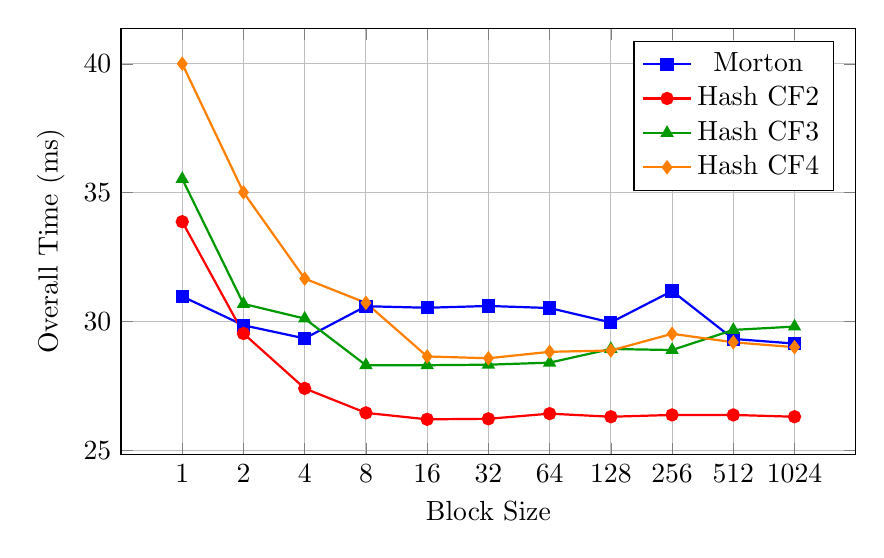
\begin{tikzpicture}
\begin{axis}[
    width=0.9\textwidth,
    height=7cm,
    xlabel={Block Size},
    ylabel={Overall Time (ms)},
    legend pos=north east,
    xmode=log,
    log basis x={2},
    xtick={1,2,4,8,16,32,64,128,256,512,1024},
    xticklabels={1,2,4,8,16,32,64,128,256,512,1024},
    grid=major,
    mark size=2pt,
]

% Morton
\addplot[color=blue,mark=square*,thick] coordinates {
    (1,30.97) (2,29.85) (4,29.34) (8,30.59) (16,30.53) 
    (32,30.60) (64,30.52) (128,29.96) (256,31.18) (512,29.32) (1024,29.14)
};

% Hash CF2
\addplot[color=red,mark=*,thick] coordinates {
    (1,33.87) (2,29.53) (4,27.40) (8,26.45) (16,26.20) 
    (32,26.22) (64,26.42) (128,26.30) (256,26.37) (512,26.37) (1024,26.30)
};

% Hash CF3
\addplot[color=green!60!black,mark=triangle*,thick] coordinates {
    (1,35.53) (2,30.68) (4,30.11) (8,28.30) (16,28.30) 
    (32,28.32) (64,28.40) (128,28.93) (256,28.89) (512,29.67) (1024,29.80)
};

% Hash CF4
\addplot[color=orange,mark=diamond*,thick] coordinates {
    (1,40.00) (2,35.01) (4,31.66) (8,30.72) (16,28.64) 
    (32,28.57) (64,28.82) (128,28.87) (256,29.52) (512,29.19) (1024,29.00)
};

\legend{Morton, Hash CF2, Hash CF3, Hash CF4}
\end{axis}
\end{tikzpicture}
\caption{Overall execution time for voxel size 0.5}
\end{figure}

% GRAPH 3: Voxel Size 0.75
\begin{figure}[H]
\centering
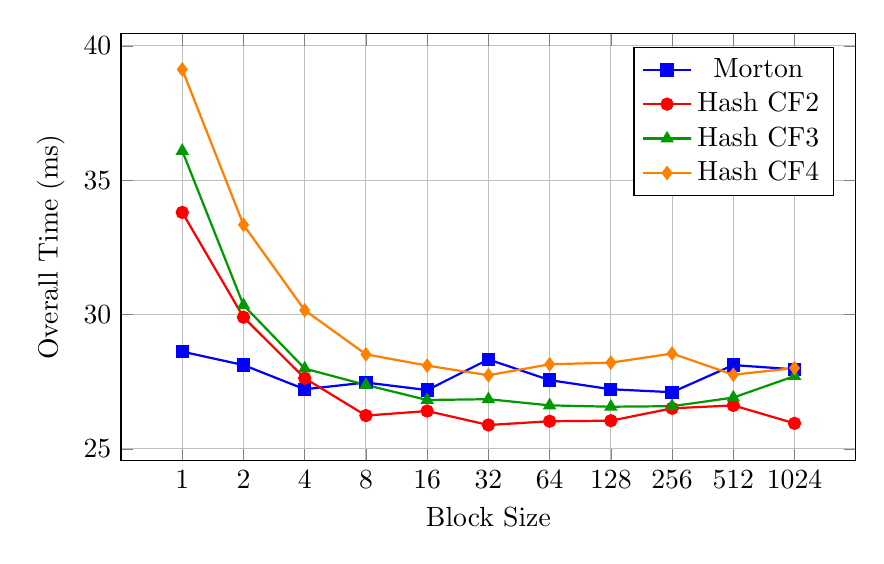
\begin{tikzpicture}
\begin{axis}[
    width=0.9\textwidth,
    height=7cm,
    xlabel={Block Size},
    ylabel={Overall Time (ms)},
    legend pos=north east,
    xmode=log,
    log basis x={2},
    xtick={1,2,4,8,16,32,64,128,256,512,1024},
    xticklabels={1,2,4,8,16,32,64,128,256,512,1024},
    grid=major,
    mark size=2pt,
]

% Morton
\addplot[color=blue,mark=square*,thick] coordinates {
    (1,28.62) (2,28.12) (4,27.22) (8,27.47) (16,27.19) 
    (32,28.33) (64,27.56) (128,27.22) (256,27.11) (512,28.12) (1024,27.96)
};

% Hash CF2
\addplot[color=red,mark=*,thick] coordinates {
    (1,33.80) (2,29.90) (4,27.63) (8,26.24) (16,26.41) 
    (32,25.89) (64,26.03) (128,26.05) (256,26.51) (512,26.62) (1024,25.95)
};

% Hash CF3
\addplot[color=green!60!black,mark=triangle*,thick] coordinates {
    (1,36.09) (2,30.35) (4,27.99) (8,27.38) (16,26.82) 
    (32,26.85) (64,26.62) (128,26.57) (256,26.59) (512,26.91) (1024,27.71)
};

% Hash CF4
\addplot[color=orange,mark=diamond*,thick] coordinates {
    (1,39.12) (2,33.34) (4,30.16) (8,28.52) (16,28.10) 
    (32,27.74) (64,28.15) (128,28.21) (256,28.55) (512,27.76) (1024,28.01)
};

\legend{Morton, Hash CF2, Hash CF3, Hash CF4}
\end{axis}
\end{tikzpicture}
\caption{Overall execution time for voxel size 0.75}
\end{figure}

% GRAPH 4: Voxel Size 1.0
\begin{figure}[H]
\centering
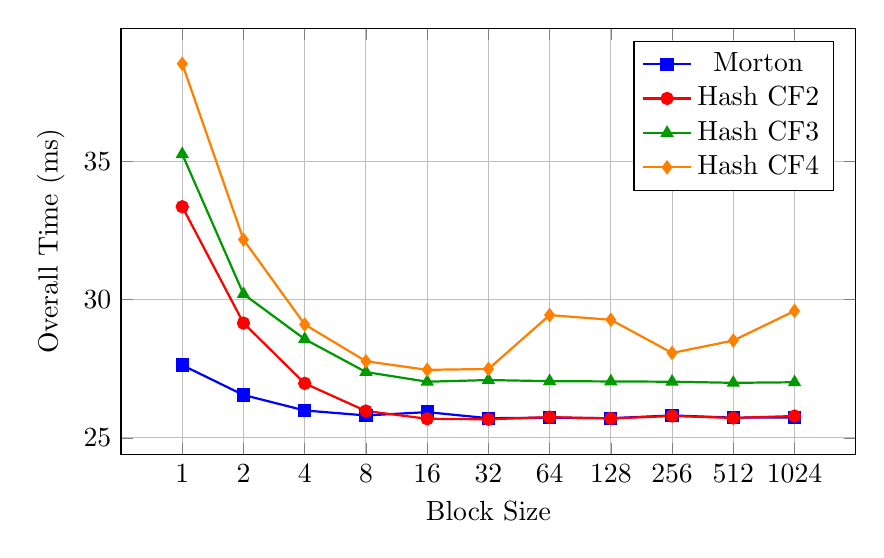
\begin{tikzpicture}
\begin{axis}[
    width=0.9\textwidth,
    height=7cm,
    xlabel={Block Size},
    ylabel={Overall Time (ms)},
    legend pos=north east,
    xmode=log,
    log basis x={2},
    xtick={1,2,4,8,16,32,64,128,256,512,1024},
    xticklabels={1,2,4,8,16,32,64,128,256,512,1024},
    grid=major,
    mark size=2pt,
]

% Morton
\addplot[color=blue,mark=square*,thick] coordinates {
    (1,27.63) (2,26.55) (4,25.99) (8,25.81) (16,25.93) 
    (32,25.71) (64,25.73) (128,25.71) (256,25.81) (512,25.73) (1024,25.74)
};

% Hash CF2
\addplot[color=red,mark=*,thick] coordinates {
    (1,33.36) (2,29.15) (4,26.97) (8,25.97) (16,25.69) 
    (32,25.67) (64,25.75) (128,25.70) (256,25.79) (512,25.72) (1024,25.79)
};

% Hash CF3
\addplot[color=green!60!black,mark=triangle*,thick] coordinates {
    (1,35.26) (2,30.20) (4,28.57) (8,27.38) (16,27.03) 
    (32,27.09) (64,27.05) (128,27.04) (256,27.03) (512,26.99) (1024,27.01)
};

% Hash CF4
\addplot[color=orange,mark=diamond*,thick] coordinates {
    (1,38.53) (2,32.17) (4,29.10) (8,27.77) (16,27.46) 
    (32,27.49) (64,29.44) (128,29.27) (256,28.07) (512,28.52) (1024,29.59)
};

\legend{Morton, Hash CF2, Hash CF3, Hash CF4}
\end{axis}
\end{tikzpicture}
\caption{Overall execution time for voxel size 1.0}
\end{figure}

% GRAPH 5: Voxel Size 1.25
\begin{figure}[H]
\centering
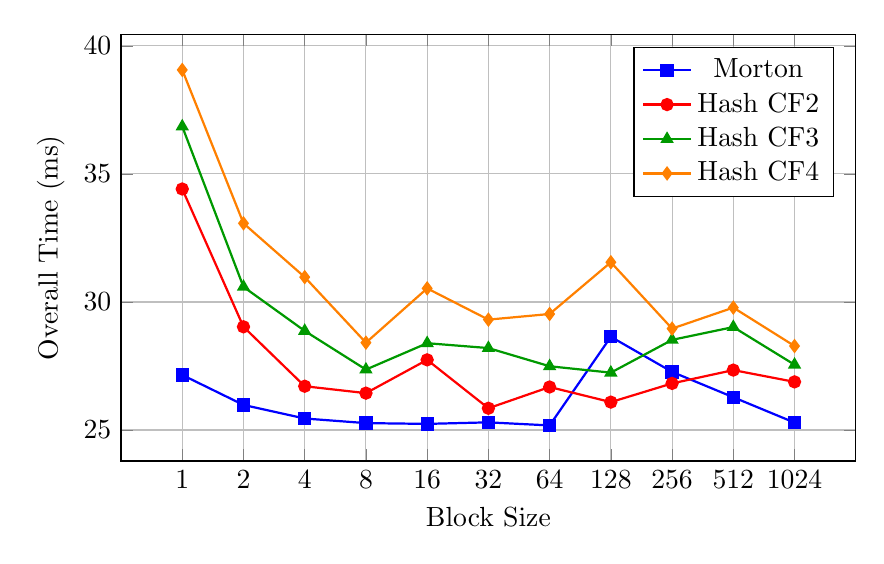
\begin{tikzpicture}
\begin{axis}[
    width=0.9\textwidth,
    height=7cm,
    xlabel={Block Size},
    ylabel={Overall Time (ms)},
    legend pos=north east,
    xmode=log,
    log basis x={2},
    xtick={1,2,4,8,16,32,64,128,256,512,1024},
    xticklabels={1,2,4,8,16,32,64,128,256,512,1024},
    grid=major,
    mark size=2pt,
]

% Morton
\addplot[color=blue,mark=square*,thick] coordinates {
    (1,27.15) (2,25.98) (4,25.45) (8,25.27) (16,25.24) 
    (32,25.30) (64,25.18) (128,28.64) (256,27.27) (512,26.28) (1024,25.29)
};

% Hash CF2
\addplot[color=red,mark=*,thick] coordinates {
    (1,34.41) (2,29.03) (4,26.71) (8,26.44) (16,27.74) 
    (32,25.85) (64,26.68) (128,26.09) (256,26.82) (512,27.34) (1024,26.88)
};

% Hash CF3
\addplot[color=green!60!black,mark=triangle*,thick] coordinates {
    (1,36.85) (2,30.59) (4,28.87) (8,27.36) (16,28.39) 
    (32,28.20) (64,27.49) (128,27.24) (256,28.52) (512,29.02) (1024,27.55)
};

% Hash CF4
\addplot[color=orange,mark=diamond*,thick] coordinates {
    (1,39.06) (2,33.07) (4,30.97) (8,28.41) (16,30.53) 
    (32,29.31) (64,29.53) (128,31.55) (256,28.96) (512,29.78) (1024,28.28)
};

\legend{Morton, Hash CF2, Hash CF3, Hash CF4}
\end{axis}
\end{tikzpicture}
\caption{Overall execution time for voxel size 1.25}
\end{figure}
\section{Visualisation}
Everything was visualised using the python open3d library. This library allows for easy loading and displaying of point clouds. The original point cloud and the voxelized point cloud were displayed side by side for comparison.
\textbf{TODOOOO : paste figures}
\section{Possible Improvements}
The main problem is that both implementations work with a fixed voxel size. This means that if the point cloud is very large but sparse, a lot of memory is wasted on empty space. A possible improvement would be to implement an octree structure, which would allow for variable voxel sizes depending on the density of points in a given area.

\begin{thebibliography}{10}
\bibitem{Nießner2013}
M. Nießner, M. Zollhöfer, S. Izadi \& M. Stamminger, “Real-time 3D Reconstruction at Scale using Voxel Hashing,” ACM Transactions on Graphics (TOG), vol. 32, no. 6, 2013.


\bibitem{morton_forceflow}
“Morton encoding/decoding through bit interleaving: Implementations”,  
Forceflow — Jeroen Baert's Blog, 7 October 2013.  
Available online: \url{https://www.forceflow.be/2013/10/07/morton-encodingdecoding-through-bit-interleaving-implementations/}  
(Accessed: 28 November 2025).

\bibitem{thrust_cccl}
NVIDIA Corporation,  
\emph{“Thrust — CUDA Core Compute Libraries (CCCL)”}.  
Available at: \url{https://nvidia.github.io/cccl/thrust/}  
(Accessed: 28 November 2025).

\bibitem{las_file_format_wikipedia}
Wikipedia contributors,  
\emph{“LAS file format”}, Wikipedia, The Free Encyclopedia.  
Available at: \url{https://en.wikipedia.org/wiki/LAS_file_format}  
(Accessed: 28 November 2025).

\bibitem{medium_voxelization}
Ayushi Sharma,  
\emph{“From Point Clouds to Voxel Grids: A Practical Guide to 3D Data Voxelization”},  
Medium, 2021.  
Available at: \url{https://medium.com/@ayushi.sharma.3536/from-point-clouds-to-voxel-grids-a-practical-guide-to-3d-data-voxelization-cf5991c1e7bb}  
(Accessed: 28 November 2025).

\end{thebibliography}
\end{document}
